\documentclass[aspectratio=169,10pt]{beamer}
\usepackage[T1]{fontenc}
\usepackage{lmodern}
\usepackage{amsmath,amssymb}
\usepackage{booktabs,tabularx}
\usepackage{graphicx}
\usepackage{tikz}
\usepackage{siunitx}
\usepackage{hyperref}
\usetikzlibrary{arrows.meta,decorations.pathmorphing}

\definecolor{ink}{HTML}{17313D}
\definecolor{accent}{HTML}{00677A}
\definecolor{warm}{HTML}{B44A25}
\definecolor{soft}{HTML}{E9F2F3}
\definecolor{muted}{HTML}{52636A}
\setbeamercolor{normal text}{fg=ink,bg=white}
\setbeamercolor{structure}{fg=accent}
\setbeamercolor{frametitle}{fg=ink,bg=white}
\setbeamercolor{block body}{bg=soft}
\setbeamerfont{frametitle}{series=\bfseries,size=\Large}
\setbeamerfont{title}{series=\bfseries,size=\Huge}
\setbeamerfont{subtitle}{size=\large}
\setbeamertemplate{navigation symbols}{}
\setbeamertemplate{itemize item}{\color{accent}$\bullet$}
\setbeamertemplate{footline}{\hbox{\begin{beamercolorbox}[wd=.86\paperwidth,ht=2.7ex,dp=1ex,leftskip=.45cm]{normal text}\scriptsize Advanced Control Theory \quad | \quad AFC: reproduction, diagnosis, extensions\end{beamercolorbox}\begin{beamercolorbox}[wd=.14\paperwidth,ht=2.7ex,dp=1ex,rightskip=.45cm plus1fil]{normal text}\hfill\scriptsize\insertframenumber/\inserttotalframenumber\end{beamercolorbox}}}
\addtobeamertemplate{frametitle}{}{\vspace{-0.6em}\textcolor{accent}{\rule{\linewidth}{0.7pt}}}
\sisetup{detect-all,per-mode=symbol}

\newcommand{\source}[1]{\vfill{\color{muted}\scriptsize #1}}
\newcommand{\takeaway}[1]{\vfill\begin{beamercolorbox}[wd=\linewidth,sep=1ex]{block body}\color{accent}\bfseries #1\end{beamercolorbox}}
\newcommand{\resfig}[3][\linewidth]{\IfFileExists{results/#2/#3.pdf}{\includegraphics[width=#1,height=0.68\textheight,keepaspectratio]{results/#2/#3.pdf}}{\includegraphics[width=#1,height=0.68\textheight,keepaspectratio]{results_octave/#2/#3.pdf}}}
\newcommand{\resfigh}[4]{\IfFileExists{results/#3/#4.pdf}{\includegraphics[width=#1,height=#2,keepaspectratio]{results/#3/#4.pdf}}{\includegraphics[width=#1,height=#2,keepaspectratio]{results_octave/#3/#4.pdf}}}

\title{Approximation-Free Active Suspension Control}
\subtitle{Na et al.\ (2022): reproduction, diagnosis and extensions}
\author{Advanced Control Theory course project}
\date{7 October 2026}

\begin{document}

\begin{frame}[plain]
\vspace{0.4cm}
{\color{accent}\rule{2.0cm}{1.2pt}}\par\vspace{0.3cm}
{\usebeamerfont{title}\inserttitle\par}
\vspace{0.3cm}
{\usebeamerfont{subtitle}\insertsubtitle\par}
\vspace{0.3cm}
\textcolor{muted}{\insertauthor\quad\textbullet\quad\insertdate}
\vfill
\begin{columns}[T]
\begin{column}{0.48\linewidth}\IfFileExists{cad/rig_preview.png}{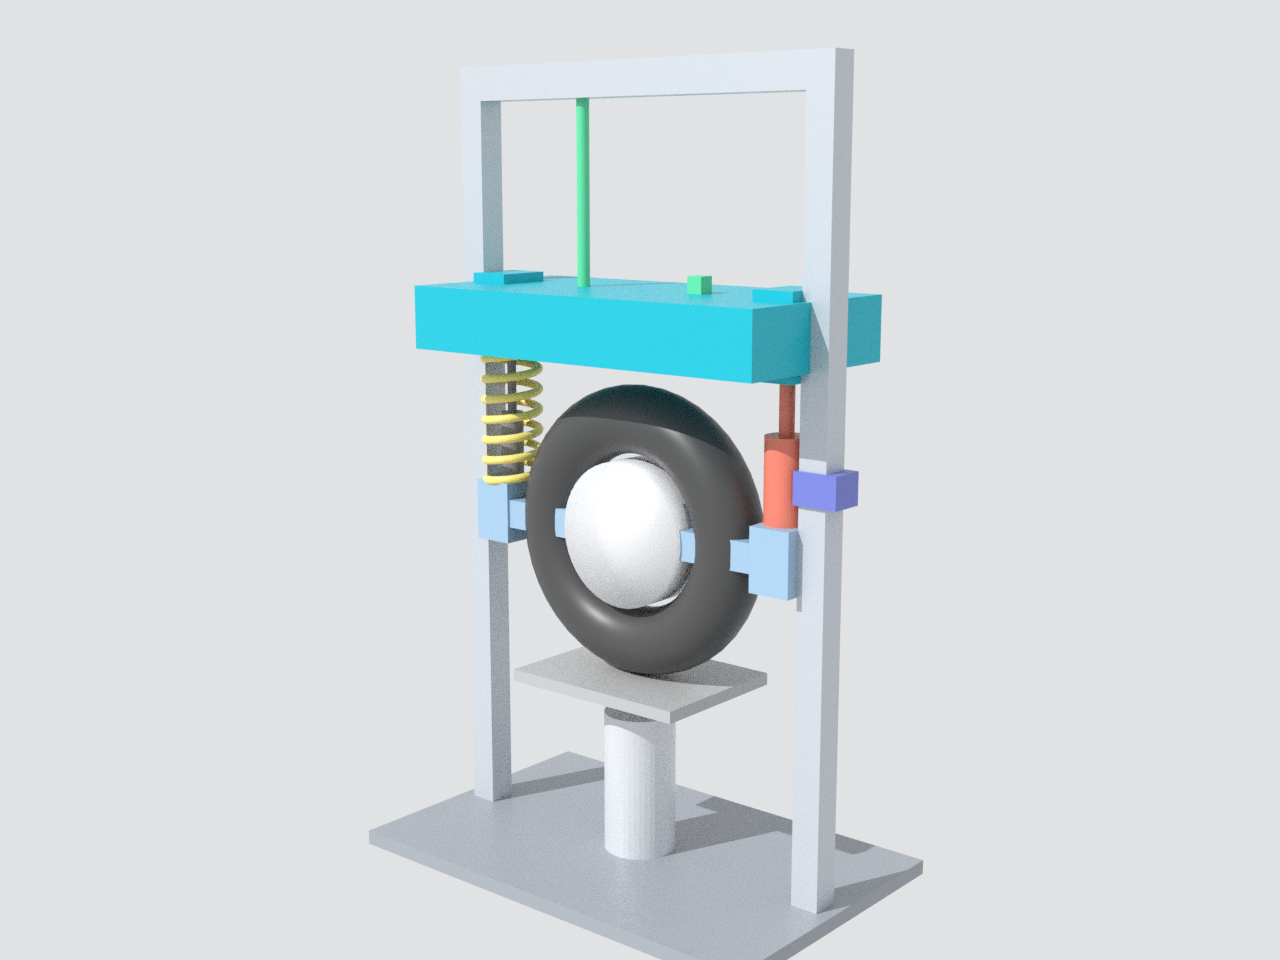
\includegraphics[height=3.3cm]{cad/rig_preview.png}}{}\end{column}
\begin{column}{0.48\linewidth}\IfFileExists{animation/preview_bump.png}{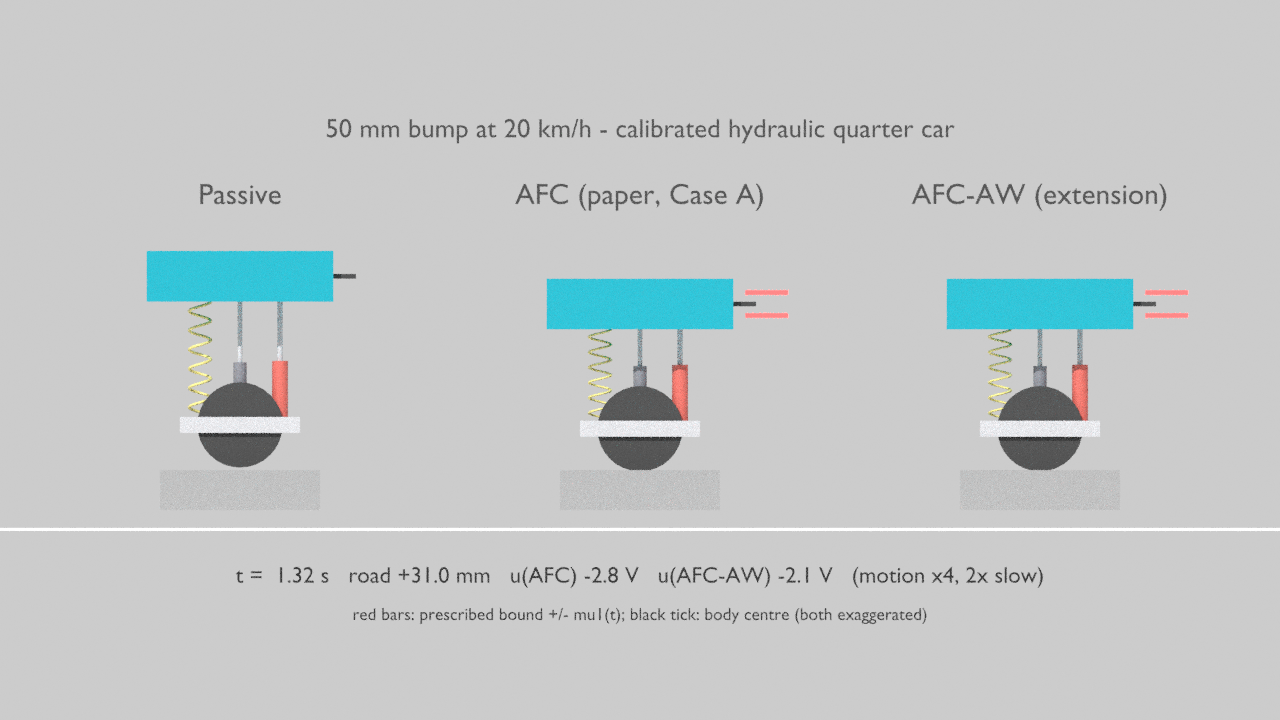
\includegraphics[height=3.0cm]{animation/preview_bump.png}}{}\end{column}
\end{columns}
\end{frame}

\begin{frame}{What we set out to answer}
\begin{columns}[T]
\begin{column}{0.48\linewidth}
{\color{accent}\large\bfseries The paper}\par\vspace{0.15cm}
Three-step approximation-free control (AFC) keeps body displacement inside a shrinking prescribed envelope; validated on a 50\,Hz electro-hydraulic rig against backstepping (BSC) and PID.
\vspace{0.25cm}

{\color{accent}\large\bfseries Our questions}\par\vspace{0.1cm}
\small\begin{enumerate}\itemsep0pt
\item What does AFC compute, and what does its proof assume?
\item Is there a plausible plant on which the paper's own gains reproduce its numbers?
\item Which claims survive sampled-data analysis, other roads, fair comparators?
\item Can the failure modes be repaired?
\end{enumerate}
\end{column}
\begin{column}{0.48\linewidth}
{\color{warm}\large\bfseries Five implementations}\par\vspace{0.15cm}
\begin{itemize}\itemsep2pt
\item MATLAB/Octave library (\texttt{afc2})
\item Simulink v2 model with sensor path
\item Simscape Multibody (mechanics from joints)
\item C on an emulated Cortex-M4
\item Browser simulator (web lab)
\end{itemize}
\vspace{0.3cm}
Each one is checked against the library.
\end{column}
\end{columns}
\source{J. Na et al., IEEE TSMC: Systems 52(8), 4714--4726, 2022. doi:10.1109/TSMC.2021.3103807.}
\end{frame}

\begin{frame}{Plant: quarter car with a servo-valve cylinder}
\begin{columns}[c]
\begin{column}{0.40\linewidth}
\centering
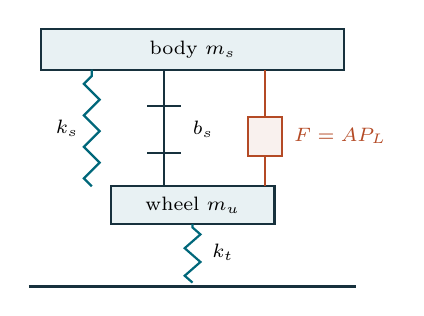
\begin{tikzpicture}[x=0.8cm,y=0.8cm,>=Stealth,thick, every node/.style={font=\scriptsize}]
  \draw[fill=accent!9,draw=ink] (1.6,3.8) rectangle (6.4,4.45); \node at (4,4.12) {body $m_s$};
  \draw[fill=accent!9,draw=ink] (2.7,1.35) rectangle (5.3,1.95); \node at (4,1.65) {wheel $m_u$};
  \draw[decorate,decoration={zigzag,segment length=4mm,amplitude=1mm},draw=accent] (2.4,1.95)--(2.4,3.8);
  \node[left] at (2.35,2.87) {$k_s$};
  \draw[draw=ink] (3.55,1.95)--(3.55,2.48); \draw[draw=ink] (3.28,2.48)--(3.82,2.48);
  \draw[draw=ink] (3.55,2.48)--(3.55,3.23); \draw[draw=ink] (3.28,3.23)--(3.82,3.23); \draw[draw=ink] (3.55,3.23)--(3.55,3.8);
  \node[right] at (3.84,2.86) {$b_s$};
  \draw[draw=warm] (5.15,1.95)--(5.15,2.43); \draw[draw=warm,fill=warm!8] (4.88,2.43) rectangle (5.42,3.05); \draw[draw=warm] (5.15,3.05)--(5.15,3.8);
  \node[right,text=warm] at (5.45,2.75) {$F=AP_L$};
  \draw[decorate,decoration={zigzag,segment length=3.5mm,amplitude=1mm},draw=accent] (4,0.42)--(4,1.35); \node[right] at (4.15,0.9) {$k_t$};
  \draw[draw=ink] (1.4,0.36)--(6.6,0.36);
\end{tikzpicture}
\end{column}
\begin{column}{0.58\linewidth}
\begin{align*}
m_s\ddot z_s&=-F_s-F_d+F,\qquad m_u\ddot z_u=F_s+F_d-F_t-F\\
\dot P_L&=-\beta P_L-\alpha A\dot d+\gamma x_v\sqrt{P_s-\operatorname{sgn}(x_v)P_L}\\
\tau\dot x_v&=-x_v+K_vu,\qquad |u|\le\SI{5}{V}
\end{align*}
State used by AFC: $x_1=z_s$, $x_2=\dot z_s$, $x_5=\kappa P_L$.\par\vspace{0.2cm}
\textcolor{warm}{Not published: $\kappa$, valve gain $K_v$, lag $\tau$.}
\end{column}
\end{columns}
\end{frame}

\begin{frame}{AFC: prescribed performance in three proportional steps}
\[
\mu_i(t)=(\mu_{i0}-\mu_{i\infty})e^{-\alpha_it}+\mu_{i\infty},\qquad
\zeta_i=\frac{e_i}{\mu_i},\qquad
\varepsilon_i=\tfrac12\ln\frac{1+\zeta_i}{1-\zeta_i}
\]
\[
e_1=x_1\to u_1=-k_1\varepsilon_1,\qquad e_2=x_2-u_1\to u_2=-k_2\varepsilon_2,\qquad e_3=x_5-u_2\to u=-k_3\varepsilon_3
\]
\vspace{0.1cm}
\begin{columns}[T]
\begin{column}{0.48\linewidth}
\small\begin{tabular}{lcccc}\toprule
Case A & $\mu_{i0}$ & $\mu_{i\infty}$ & $\alpha_i$ & $k_i$\\\midrule
$z_s$ & 0.2 & 0.018 & 3 & 25.5\\ virtual vel. & 110 & 90 & 2 & 12\\ pressure & 100 & 80 & 2 & 216\\\bottomrule
\end{tabular}
\end{column}
\begin{column}{0.48\linewidth}
\textbf{Proof (Lemma 1):} bounded $\varepsilon_i\Rightarrow|\zeta_i|\le\tanh\varepsilon_{Mi}<1$.\par
Assumes \textcolor{warm}{continuous time}, \textcolor{warm}{unsaturated input}, bounded $F_i$. Promises ultimate boundedness, not convergence.
\end{column}
\end{columns}
\takeaway{No derivatives of virtual controls, no model terms. But the gains are numbers in the rig's units.}
\end{frame}

\begin{frame}{Baseline diagnosis: the paper's gains on our first plant}
\begin{columns}[T]
\begin{column}{0.46\linewidth}
\begin{itemize}\itemsep4pt
\item v1 plant: assumed first-order actuator. AFC saturated 85\%, envelope crossed by 18.9\,mm.
\item Linearised 50\,Hz loop: $u\approx-510z_s-0.36\dot z_s-2.70x_5$, spectral radius \textbf{1.02}, so \textcolor{warm}{unstable}.
\item Remove the $\pm5$\,V rail: IAE 0.48$\to$2.37, body moves 0.23\,m.
\item No actuator gain $b_u$ fixes it.
\end{itemize}
\end{column}
\begin{column}{0.52\linewidth}\centering\resfig{phase1}{fig_stability}\end{column}
\end{columns}
\takeaway{Saturation was limiting the instability, not causing it. The gains do not fit this plant's scale.}
\end{frame}

\begin{frame}{A literature plant, calibrated on one paper experiment}
\begin{columns}[T]
\begin{column}{0.44\linewidth}
\begin{itemize}\itemsep4pt
\item Alleyne--Hedrick hydraulic quarter car (290/59\,kg, servo-valve law).
\item Free: valve gain $K_v$ and lumped lag $\tau$. Grid fit to the paper's Case-10 AFC indices.
\item Best: $K_v=5\times10^{-4}$\,m/V, $\tau=33$\,ms, error 4\%.
\item Literature spool lag (3\,ms): error 62--69\%.
\end{itemize}
\end{column}
\begin{column}{0.54\linewidth}\small
\resizebox{\linewidth}{!}{\IfFileExists{results/phase1/case10_table.tex}{% Generated by run_phase1.m -- calibrated plant, paper Case A gains
\begin{tabular}{lrrrrrrrr}
\toprule
 & \multicolumn{2}{c}{IAE (m\,s)} & \multicolumn{2}{c}{ITAE (m\,s$^2$)} & \multicolumn{2}{c}{ITSE (m$^2$s$^2$)} & \multicolumn{2}{c}{$u_{\mathrm{RMS}}$ (V)}\\
Controller & sim & paper & sim & paper & sim & paper & sim & paper$^\ast$\\
\midrule
AFC & 0.1294 & 0.1216 & 1.197 & 1.140 & 0.0088 & 0.0093 & 0.50 & 0.5\\
BSC & 0.6756 & 0.2108 & 6.864 & 1.952 & 0.3101 & 0.0224 & 4.98 & 4.7\\
PID & 0.8059 & 0.1881 & 8.829 & 1.191 & 0.5517 & 0.0219 & 4.98 & 5.0\\
Passive & 0.6661 & -- & 6.651 & -- & 0.2744 & -- & 0.00 & --\\
\bottomrule
\end{tabular}
}{% Generated by run_phase1.m -- calibrated plant, paper Case A gains
\begin{tabular}{lrrrrrrrr}
\toprule
 & \multicolumn{2}{c}{IAE (m\,s)} & \multicolumn{2}{c}{ITAE (m\,s$^2$)} & \multicolumn{2}{c}{ITSE (m$^2$s$^2$)} & \multicolumn{2}{c}{$u_{\mathrm{RMS}}$ (V)}\\
Controller & sim & paper & sim & paper & sim & paper & sim & paper$^\ast$\\
\midrule
AFC & 0.1294 & 0.1216 & 1.197 & 1.140 & 0.0088 & 0.0093 & 0.50 & 0.5\\
BSC & 0.6756 & 0.2108 & 6.864 & 1.952 & 0.3101 & 0.0224 & 4.98 & 4.7\\
PID & 0.8059 & 0.1881 & 8.829 & 1.191 & 0.5517 & 0.0219 & 4.98 & 5.0\\
Passive & 0.6661 & -- & 6.651 & -- & 0.2744 & -- & 0.00 & --\\
\bottomrule
\end{tabular}
}}
\par\vspace{0.2cm}{\scriptsize paper$^\ast$: read from Fig.~13 by eye}
\end{column}
\end{columns}
\takeaway{The paper's unchanged AFC reproduces IAE/ITAE/ITSE within 7\% and its sub-volt command. BSC and PID saturate, as reported.}
\end{frame}

\begin{frame}{Case 10: displacement and command}
\begin{columns}[T]
\begin{column}{0.5\linewidth}\centering\resfig{phase1}{fig_case10_displacement}\end{column}
\begin{column}{0.5\linewidth}\centering\resfig{phase1}{fig_case10_control}\end{column}
\end{columns}
\source{Compare the paper's Figs.~6 and 10. All traces are simulation.}
\end{frame}

\begin{frame}{Is it the code? Four implementations, one answer}
\begin{columns}[T]
\begin{column}{0.55\linewidth}\centering
\IfFileExists{results/phase2/simulink_v2_ideal.png}{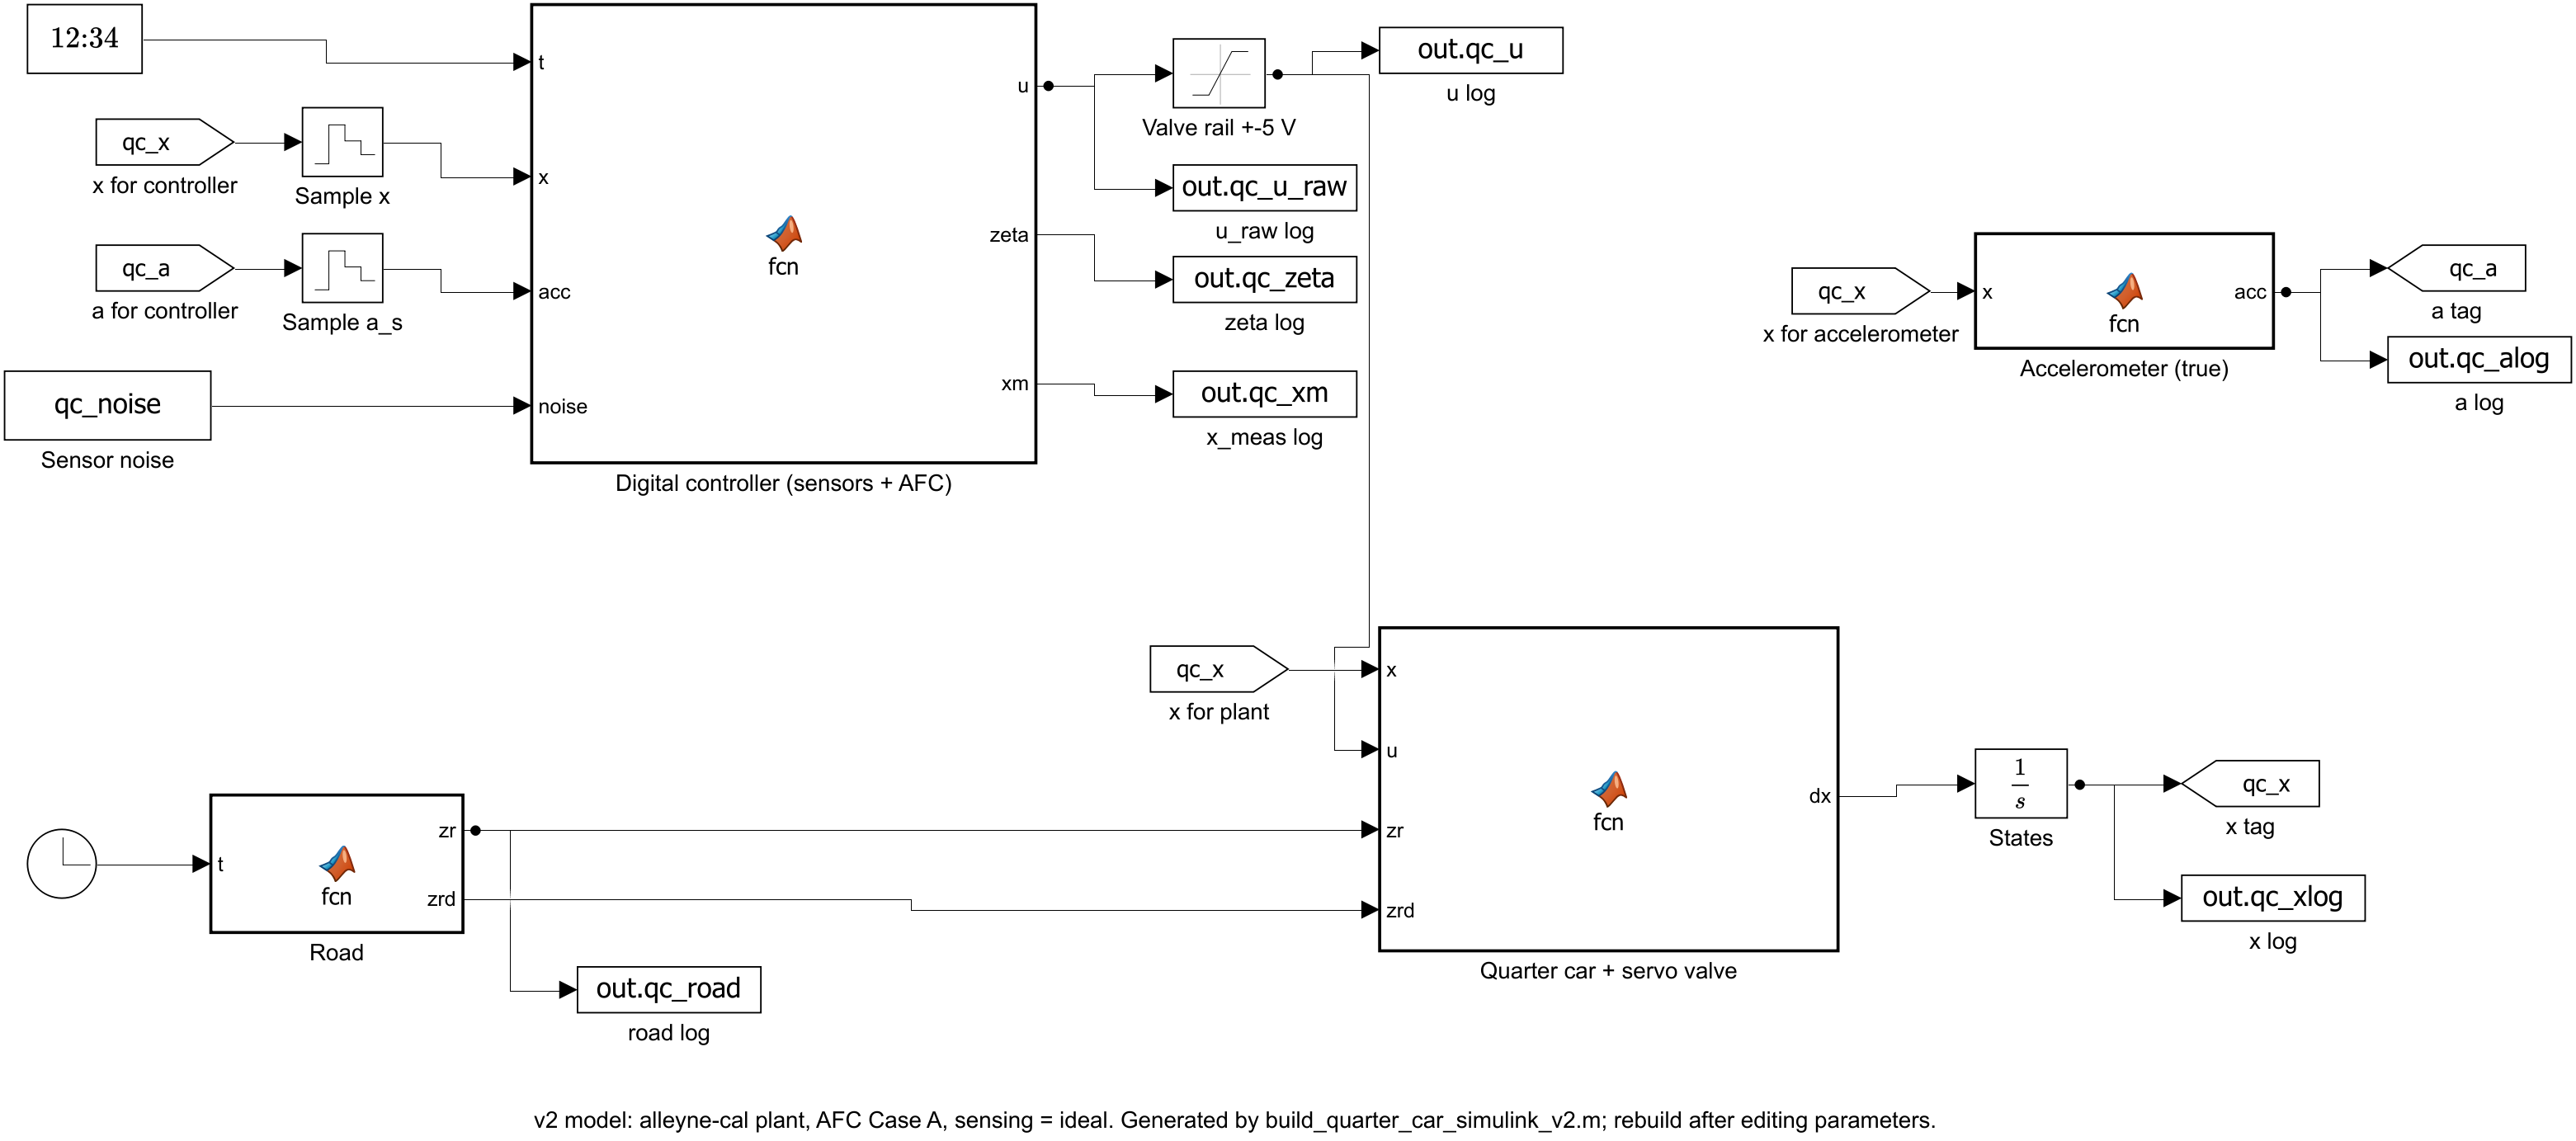
\includegraphics[width=\linewidth,height=0.33\textheight,keepaspectratio]{results/phase2/simulink_v2_ideal.png}}{}\par
{\scriptsize Simulink v2: 50\,Hz digital controller, $\pm5$\,V rail, servo-valve plant}\par\vspace{0.1cm}
\footnotesize\begin{tabular}{@{}lr@{}}\toprule
Check against the \texttt{afc2} equations & max $|\Delta z_s|$\\\midrule
Simulink v2 (same sensor noise) & $4\times10^{-16}$\,m\\
Simscape Multibody (joints, \texttt{ode15s}) & 2.1\,$\mu$m\\
C on Cortex-M4 (control law) & 10 digits\\
MATLAB R2026a vs Octave 8.4 & same digits$^\dagger$\\\bottomrule
\end{tabular}
\end{column}
\begin{column}{0.43\linewidth}\centering\resfig[\linewidth]{phase2b}{fig_multibody_crosscheck}\par{\scriptsize Case 10, AFC Case A: $z_s$ from equations (RK4) and Multibody (\texttt{ode15s})}\end{column}
\end{columns}
{\color{muted}\tiny $^\dagger$ except saturated Case-B runs: on the rail, rounding picks the limit cycle.}
\takeaway{Multibody builds the mechanics from joints, not our equations, and agrees to 2\,$\mu$m.}
\end{frame}

\begin{frame}{Hold-out: can any plant explain both gain sets?}
\begin{columns}[T]
\begin{column}{0.52\linewidth}\centering\resfig{phase1}{fig_sweep_holdout}\end{column}
\begin{column}{0.46\linewidth}
\begin{itemize}\itemsep4pt
\item AFC lowest IAE on all 8 roads, as in the paper.
\item But Case-B gains saturate (4.1--4.4\,V RMS vs the paper's $\approx$0.45\,V).
\item Joint fit of $\kappa,K_v,\tau$ on roads 10/A and 6/B: train error 0.22, \textbf{test error 0.63}.
\end{itemize}
\end{column}
\end{columns}
\takeaway{The paper does not publish enough to identify its rig. Compare trends, not digits.}
\end{frame}

\begin{frame}{Where Lemma 1 holds and where it fails}
\begin{columns}[T]
\begin{column}{0.56\linewidth}\centering\resfig{phase3}{fig_lyapunov}\end{column}
\begin{column}{0.42\linewidth}
\begin{itemize}\itemsep4pt
\item Calibrated: $\max|\zeta_1|=0.50$, $\varepsilon_{M1}=0.555$, bound $\tanh\varepsilon_{M1}=0.504$. Tight.
\item v1: $|\zeta|\ge1$ in 69.5\% of samples and \textbf{every one} is saturated.
\end{itemize}
\end{column}
\end{columns}
\takeaway{The conclusion fails exactly where the unsaturated-input assumption fails.}
\end{frame}

\begin{frame}{Near zero error, AFC is a skyhook spring}
\begin{columns}[T]
\begin{column}{0.46\linewidth}
\[u\approx-\tfrac{k_3}{\mu_3}\Big(x_5+\tfrac{k_2}{\mu_2}\big(\dot z_s+\tfrac{k_1}{\mu_1}z_s\big)\Big)\]
\begin{itemize}\itemsep4pt
\item Skyhook spring 63\,kN/m, skyhook damper only 45\,N\,s/m.
\item The barrier stiffens the spring as $|z_s|\to\mu_1$.
\item Body motion 0.22 of road at 0.5\,Hz (passive 1.22); 4--8\,Hz acceleration about $2\times$ passive.
\end{itemize}
\end{column}
\begin{column}{0.52\linewidth}\centering\resfig{phase3}{fig_frequency_response}\end{column}
\end{columns}
\end{frame}

\begin{frame}{The continuous proof misses a sampled-data instability}
\begin{columns}[T]
\begin{column}{0.46\linewidth}
\begin{itemize}\itemsep4pt
\item Continuous linearised loop: stable (slowest pole $-1.71\pm15.7j$).
\item Any ZOH, 1--20\,ms: unstable (spectral radius 1.03--4.4).
\item Cause: lightly damped 88\,Hz hydraulic mode under pressure feedback.
\item Nonlinear result: bounded 0.13\,mm oscillation at $\approx$12\,Hz, which fits the paper's ``residual oscillations''.
\end{itemize}
\end{column}
\begin{column}{0.52\linewidth}\centering\resfig{phase1}{fig_stability}\end{column}
\end{columns}
\end{frame}

\begin{frame}{Fair comparators at equal effort}
\begin{columns}[T]
\begin{column}{0.56\linewidth}\centering\resfig{phase3}{fig_tradeoff}\end{column}
\begin{column}{0.42\linewidth}
\begin{itemize}\itemsep4pt
\item At AFC's 0.5\,V RMS: skyhook IAE \textbf{0.086}, LQR \textbf{0.071}, AFC 0.129.
\item AFC gains $\times\tfrac12$: 81\% saturation; $\times2$: 96\%. Only a narrow window works.
\item BSC/PID with paper gains: saturated, worse than passive here.
\end{itemize}
\end{column}
\end{columns}
\takeaway{AFC's advantage is the explicit bound and no model, not efficiency.}
\end{frame}

\begin{frame}{Robustness and transients}
\begin{columns}[T]
\begin{column}{0.44\linewidth}\centering\resfig{phase3}{fig_monte_carlo}\end{column}
\begin{column}{0.54\linewidth}\centering\resfigh{\linewidth}{0.58\textheight}{phase3}{fig_bump_iso}\end{column}
\end{columns}
\takeaway{AFC keeps the bound on 37/40 plants (BSC, PID: 0/40). On a 50\,mm bump it switches rail to rail; tyre load 1.77$\times$ static, so the wheel leaves the road.}
\end{frame}

\begin{frame}{Extension: let the envelope breathe under saturation}
\[\mu_{i,\rm eff}=\mu_i(t)(1+\rho),\qquad \dot\rho=-0.5\rho+5\,\frac{|u_{\rm raw}-\operatorname{sat}(u_{\rm raw})|}{V_{\max}}\]
\begin{columns}[T]
\begin{column}{0.46\linewidth}
\begin{itemize}\itemsep4pt
\item Same law, still model-free, one extra state.
\item Bump: peak 18.8\,mm, 0\% saturation, tyre load 0.73.
\item Case 10: identical to AFC (never saturates).
\item Half car: heave acceleration 6.6$\to$1.3\,m/s$^2$.
\end{itemize}
\end{column}
\begin{column}{0.52\linewidth}\centering\resfigh{\linewidth}{0.62\textheight}{phase3b}{fig_halfcar_bump}\end{column}
\end{columns}
\end{frame}

\begin{frame}{Implementation realism: sensors and computation time}
\begin{columns}[T]
\begin{column}{0.48\linewidth}
{\color{accent}\bfseries Sensing (paper: $z_s$ and $\ddot z_s$ only)}
\begin{itemize}\itemsep3pt
\item Velocity by integration beats differencing: 0.025 vs 0.034\,m/s.
\item Noise doubles to triples the acceleration RMS; at 4$\times$ noise it reaches 1.1\,m/s$^2$ (paper: 1.67).
\end{itemize}
\end{column}
\begin{column}{0.50\linewidth}
{\color{accent}\bfseries Cortex-M4, no FPU (paper's MK60D)}\par\small
\begin{tabular}{lrrr}\toprule & instr./call & est.\ ms & paper ms\\\midrule
AFC & 18\,070 & 0.18--0.27 & 4.2\\ BSC & 9\,275 & 0.09--0.14 & 5.8\\ PID & 940 & 0.01 & 2.6\\\bottomrule\end{tabular}
\end{column}
\end{columns}
\takeaway{The law alone costs AFC about 2$\times$ BSC. The paper's timing advantage comes from elsewhere in its loop.}
\end{frame}

\begin{frame}{Verdicts on the paper's claims}
\small
\begin{tabularx}{\linewidth}{@{}lXl@{}}\toprule
Claim & Evidence & Verdict\\\midrule
Stays inside the PPF & Holds unsaturated (Case 10); fails on v1, bumps, ISO roads & \textcolor{warm}{Conditional}\\
Beats BSC and PID & Reproduced with paper gains; LQR/skyhook match it at equal effort & Reproduced\\
Small, smooth command & 0.5\,V RMS vs $\approx$5\,V & Reproduced\\
No model needed & Law yes; gains are plant-scale specific & Qualified\\
Proof covers the rig & Continuous only; 50\,Hz loop locally unstable, bounded & Qualified\\
Cheaper than BSC & Not at law level (2$\times$ instructions) & \textcolor{warm}{Not supported}\\
Integrate acc.\ for velocity & Supported & Reproduced\\\bottomrule
\end{tabularx}
\end{frame}

\begin{frame}{Tools: CAD rig, Blender animation, web lab}
\begin{columns}[T]
\begin{column}{0.32\linewidth}\centering\IfFileExists{cad/rig_preview.png}{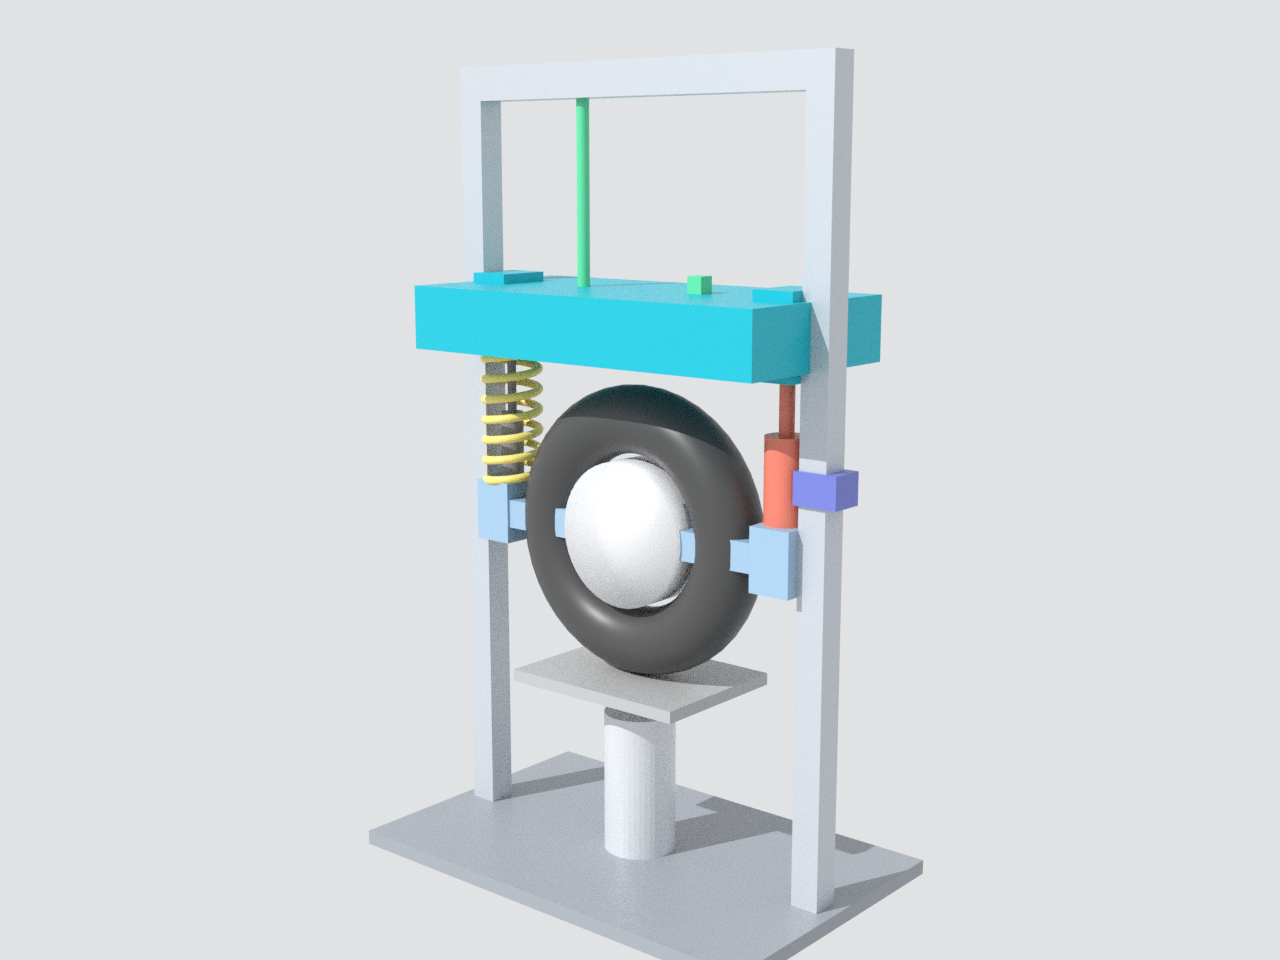
\includegraphics[width=\linewidth]{cad/rig_preview.png}}{}\par\scriptsize FreeCAD macro $\to$ STEP/STL
\end{column}
\begin{column}{0.64\linewidth}\centering\IfFileExists{animation/preview_bump.png}{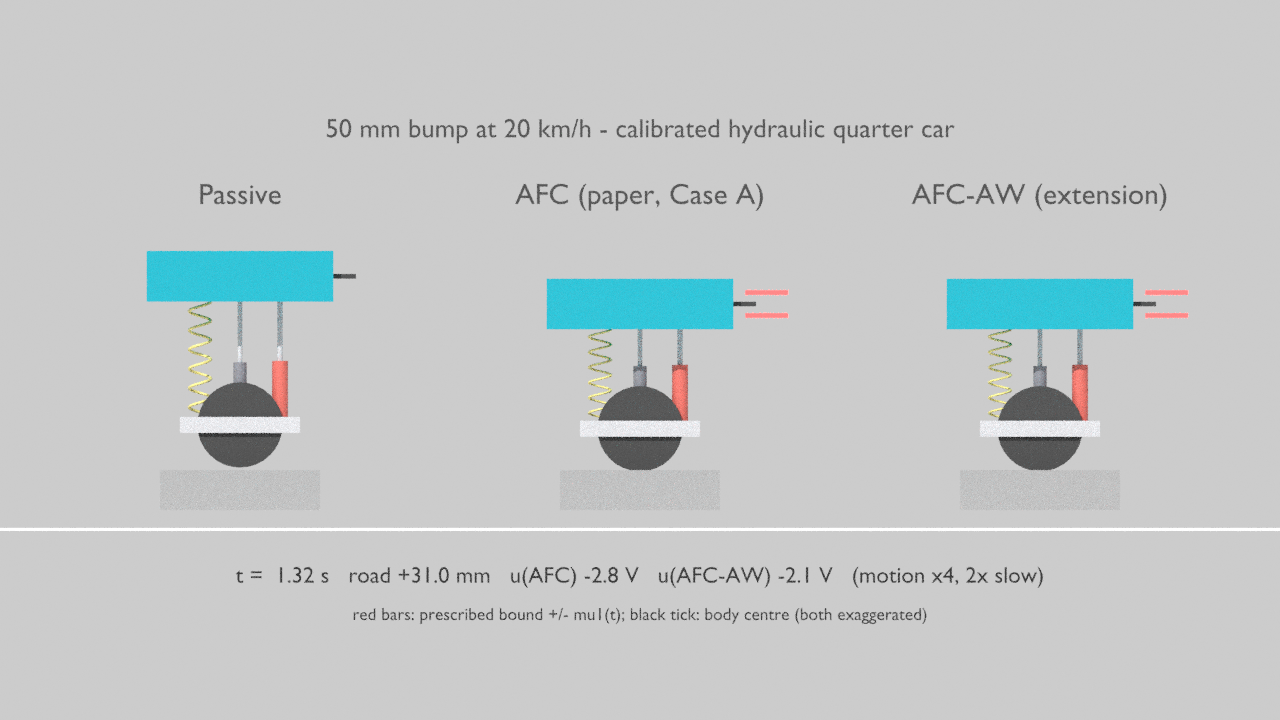
\includegraphics[width=\linewidth]{animation/preview_bump.png}}{}\par\scriptsize Blender, driven by simulated trajectories (passive | AFC | AFC-AW)\end{column}
\end{columns}
\source{Interactive web lab: same equations in the browser, sliders for gains, envelope, valve and road.}
\end{frame}

\begin{frame}{Conclusions}
\begin{itemize}\itemsep6pt
\item AFC puts a transient specification into a very simple law, and its proof says when it works: when the actuator can deliver what the barrier asks for.
\item With a calibrated literature plant, the paper's own gains reproduce its headline numbers and ranking.
\item The gains are tied to the plant's scale. The 50\,Hz loop is locally unstable but bounded, linear designs match it at equal effort, and transients drive it into saturation.
\item Envelope relaxation keeps the method's simplicity and removes the bump failure, in quarter and half car.
\item To go further we would need the rig's valve gain, effective lag and pressure scaling. Everything here re-runs with them unchanged.
\end{itemize}
\source{Code, models, figures: github.com/Galabavamsi/quarter-car-afc-replication}
\end{frame}

\end{document}
